% !TeX program = xelatex
% Цитаты только из ../../tex/5/chapter.tex и отдельно разрешённого пользователем ../../tex/5/notes.tex.
\documentclass[12pt,a4paper]{article}
\usepackage{fontspec}
\setmainfont{Times New Roman}
\usepackage[english,russian]{babel}
\usepackage{amsmath,amssymb}
\usepackage[margin=22mm]{geometry}
\usepackage{graphicx,float}
\usepackage[unicode,hidelinks]{hyperref}
\DeclareMathOperator{\grad}{grad}
\setlength{\emergencystretch}{3em}
\interfootnotelinepenalty=10000
\setlength{\parindent}{0pt}
\renewcommand{\thefootnote}{\arabic{footnote})}
\newcommand{\topic}[1]{\par\medskip\noindent\textbf{#1}\par\nobreak\smallskip}
\newenvironment{textquote}{\begin{quote}\sloppy}{\end{quote}}
\newcommand{\source}[1]{\par\nobreak\smallskip{\small Н. Е. Леонтьев. \textit{Основы теории фильтрации}. 2-е изд., 2017. Глава II, §~8, с.~#1.}\par\medskip}
\begin{document}
\section*{Вопрос 5}
\noindent Плоская установившаяся фильтрация несжимаемой жидкости. Типичные постановки задач. Применение методов ТФКП. Примеры: постановка задачи о водонепроницаемой плотине с плоским основанием; постановка задачи о работе кротового оросителя.

\medskip
\noindent\textbf{Источники:} Н. Е. Леонтьев. \textit{Основы теории фильтрации}. 2-е изд. Москва: МАКС Пресс, 2017. Глава II, § 8, печатные страницы 43--54. Для трубы-источника отдельно включён фрагмент \textit{рукописного конспекта лекций}, файл \texttt{porous-lecture-notes.pdf}, страницы PDF 14--15; автор и год не указаны. Ниже приведены дословные цитаты перенесённых в TeX материалов.
\par\bigskip
% Цитата 1; печатные страницы: 43
\begin{textquote}
Во многих практически важных случаях фильтрационные течения можно приближенно рассматривать как \textit{плоскопараллельные}, что дает возможность перейти от трехмерной задачи к двумерной и позволяет, как и в случае плоских течений идеальной несжимаемой жидкости, эффективно использовать аппарат теории функций комплексного переменного.

Типичный пример таких явлений --- движение жидкости в поперечных сечениях протяженных объектов: фильтрация под плотинами гидроэлектростанций и другими гидротехническими сооружениями (рис. 1), просачивание жидкости через земляные плотины (рис. 9~\textit{а}), отток жидкости через дно рек и каналов и т.п. Другим важным примером явлений, в которых применима модель плоскопараллельного течения, служит фильтрация в горизонтальных пластах в недрах земли. Образно выражаясь, в первом случае фильтрационное течение рассматривается при взгляде «сбоку», а во втором случае --- при взгляде «сверху».
\source{43}
\end{textquote}

% Цитата 2; печатные страницы: 44--45
\begin{textquote}
Рассмотрим плоское фильтрационное течение тяжелой несжимаемой жидкости в вертикальном поперечном сечении \textit{однородной} пористой среды. Направив оси $x$ и $y$ соответственно горизонтально и вертикально, можно записать систему уравнений в виде
\[
\triangle\varphi(x,y)=0,\qquad \boldsymbol{u}=(u(x,y);v(x,y))=\grad\varphi,
\]
где введен \textit{потенциал скорости фильтрации}
\begin{equation}
\varphi(x,y)\equiv-CH=-C\left(\frac{p(x,y)}{\rho g}+y\right),\qquad C=\mathrm{const}.
\tag{8.1}\label{q5:eq-8-1}
\end{equation}
Задача свелась к нахождению решения двумерного уравнения Лапласа, поэтому удобно рассматривать плоскость $Oxy$ как плоскость комплексного переменного $z=x+iy$, а потенциал $\varphi$ --- как действительную часть \textit{комплексного потенциала течения} --- аналитической функции $w(z)=\varphi(x,y)+i\psi(x,y)$, где $\psi(x,y)$ --- \textit{функция тока}, удовлетворяющая уравнениям Коши--Римана (Д’Аламбера--Эйлера) [9]
\[
\frac{\partial\varphi}{\partial x}=\frac{\partial\psi}{\partial y},\qquad
\frac{\partial\varphi}{\partial y}=-\frac{\partial\psi}{\partial x}.
\]
Задание комплексного потенциала полностью определяет фильтрационное течение, т.к. зная $w(z)$ можно найти распределение давления из (8.1) и распределение скорости фильтрации с помощью формулы $\frac{dw}{dz}=v-iu$, поэтому решение конкретной краевой задачи сводится к нахождению функции $w(z)$, удовлетворяющей заданным краевым условиям на границах области течения (известных или неизвестных).

Основная идея применения методов комплексного анализа при нахождении функции $w(z)$ состоит в том, что по известным условиям на границе области (в физической плоскости $z$) можно сразу сказать, каким условиям будет удовлетворять образ границы при отображениях $w(z)$, $\frac{dw(z)}{dz}$ или каких-то других (например, в зависимости от типа границы, указать значение мнимой части $w(z)$ или найти связь действительной и мнимой частей $\frac{dw(z)}{dz}$). Основываясь на этой информации можно построить конформное отображение области течения на какой-либо из ее образов или (если
область течения заранее неизвестна) найти отображение одного образа на другой. Это конформное отображение дает либо сразу искомую функцию (если область в плоскости $z$ отображается на плоскость $w$), либо обыкновенное дифференциальное уравнение, из которого находится $w(z)$.
\source{44--45}
\end{textquote}

% Цитата 3; печатные страницы: 45
\begin{textquote}
На непроницаемой границе, так же как и в гидродинамике идеальной несжимаемой жидкости, постоянна мнимая часть комплексного потенциала: $\operatorname{Im}w=\psi=\mathrm{const}$. Значение константы на конкретной поверхности может либо определяться из условия задачи\footnote[1]{Напомним, что разность значений функции тока в двух точках (внутри односвязной области) равна расходу жидкости через любую кривую, соединяющую точки.}, либо находиться из решения. В силу того, что функция тока определена с точностью до константы (физический смысл имеют ее пространственные производные), значение $\psi$ в одной точке можно задать произвольно.

Если участок границы является \textit{прямолинейным}, то вектор скорости фильтрации направлен вдоль границы. Поэтому в плоскости годографа\footnote[2]{Годограф (греч. $o\delta o\varsigma$ --- «путь», «движение», $\gamma\rho\alpha\varphi\omega$ --- «пишу») --- геометрическое место концов векторов скорости, откладываемых от начала координат. Плоскость годографа $(u;v)$ получается из плоскости $\frac{dw}{dz}=(u;-v)$ отражением относительно горизонтальной оси.} этой границе соответствует прямая, проходящая через начало координат и параллельная\footnote[3]{Если считать совпадающими ориентации осей координатных систем $(x;y)$ и $(u;v)$.} границе.
\source{45}
\end{textquote}

% Цитата 4; печатные страницы: 45--46
\begin{textquote}
На границах этого типа значение напора $H$, а следовательно, и потенциала $\varphi$, является постоянной величиной. Действительно, если свободная поверхность жидкости в водоеме имеет вертикальную координату $y=h$, то в любой точке внутри водоема, в том числе и на границе с пористой средой,
\[
H(x,y)=\frac{p_{\text{атм}}+\rho g(h-y)}{\rho g}+y=p_{\text{атм}}+\rho gh=\mathrm{const}.
\]
Постоянство $\varphi$ на границе приводит, вследствие закона Дарси,
к тому, что вектор скорости фильтрации перпендикулярен границе (т.к. его касательная составляющая равна нулю). Поэтому \textit{прямолинейной} границе этого типа на плоскости годографа соответствует прямая, проходящая через начало координат и перпендикулярная направлению границы.
\source{45--46}
\end{textquote}

% Цитата 5; печатные страницы: 46
\begin{textquote}
В случае \textit{стационарной} фильтрации поверхность депрессии является линией тока, и на ней функция тока постоянна: $\psi=\mathrm{const}$\footnote[1]{В \textit{нестационарном} случае, когда скорость границы $D$ отлична от нуля, функция тока переменна вдоль границы: из условия на разрыве $mD=u_n=\pm\bigl(\frac{\partial\psi}{\partial y}\cdot\frac{dy}{ds}+\frac{\partial\psi}{\partial x}\cdot\frac{dx}{ds}\bigr)=\pm\frac{d\psi}{ds}$, где $s$ --- длина дуги вдоль границы (знак перед производной зависит от выбора направления вдоль границы и знака $D$).}.

Уравнение образа свободной поверхности на плоскости годографа проще всего получить с помощью условия $u_n=mD$, отвечающего сохранению массы на разрыве. Если граница задается уравнением $f(x,y,t)=0$, то это условие дает
\[
\frac{\grad\varphi\cdot\grad f}{|\grad f|}=-m\frac{\dfrac{\partial f}{\partial t}}{|\grad f|},\qquad
\grad f=\left(\frac{\partial f}{\partial x};\frac{\partial f}{\partial y}\right),
\]


или
\[
m\frac{\partial f}{\partial t}+\grad f\cdot\grad\varphi=0.
\]
Воспользовавшись постоянством давления на свободной поверхности и определением потенциала (8.1), можно написать уравнение свободной поверхности в виде
\[
f(x,y,t)\equiv\varphi(x,y,t)+Cy+\mathrm{const}=0,
\]
подстановка которого в предыдущее уравнение дает условие на границе в нестационарном случае
\[
m\frac{\partial\varphi}{\partial t}+\left(\frac{\partial\varphi}{\partial x}\right)^2+\left(\frac{\partial\varphi}{\partial y}\right)^2+C\frac{\partial\varphi}{\partial y}=0.
\]
Отсюда при стационарной фильтрации на плоскости годографа получаем окружность радиуса $C/2$, проходящую через начало координат (рис.~14):
\[
u^2+v^2+Cv=0.
\]
\source{46}
\end{textquote}

% Цитата 6; печатные страницы: 47
\begin{textquote}
Для поверхности высачивания написать условие на потенциал $w$, не содержащее координат $x$, $y$, не удается, а в плоскости годографа образ границы можно построить в случае \textit{прямолинейной} границы. Умножая закон Дарси
\[
\boldsymbol{u}=-C\grad\left(\frac{p}{\rho g}+y\right)
\]
на касательный вектор к границе $\boldsymbol{\tau}$, получим, учитывая постоянство давления вдоль границы,
\[
\boldsymbol{u}\cdot\boldsymbol{\tau}=-C\tau_y=\mathrm{const},
\]
т.е. на плоскости $(u;v)$ концы вектора скорости лежат на прямой, перпендикулярной границе, но не проходящей, вообще говоря, через начало координат.
\source{47}
\end{textquote}

% Цитата 7; печатные страницы: 47--48
\begin{textquote}
\topic{Непроницаемая плотина с плоским основанием на пористом слое бесконечной глубины}
Рассмотрим стационарную фильтрацию жидкости через слой пористого материала, на котором находится непроницаемая плотина с плоским основанием длиной $2l$. Выберем начало координат в середине основания плотины (см. рис.~15) и будем считать, что уровни жидкости $h_1$ и $h_2$ соответственно в нижнем и верхнем бьефах постоянны, а пористый слой простирается вниз до бесконечности.

\setcounter{figure}{14}
\begin{figure}[H]
\centering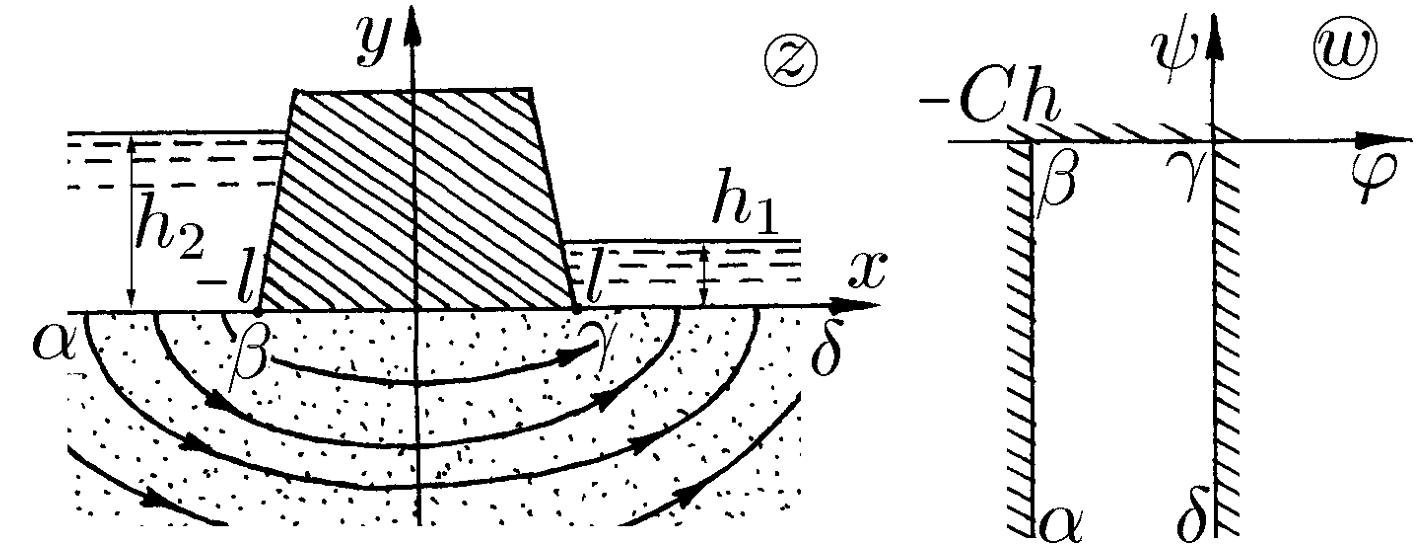
\includegraphics[width=.85\linewidth]{figures/figure-15.png}
\caption{}\label{q5:fig-15}
\end{figure}
В этой задаче область течения в плоскости комплексного потенциала $w$ полностью определена и является полубесконечной полосой: на непроницаемом основании плотины $\beta\gamma$ постоянна функция тока $\psi$, которую можно положить равной нулю, а на
дне каждого из водоемов потенциалы скорости фильтрации $\varphi$ принимают постоянные значения. Если значение $\varphi$ на дне $\gamma\delta$ в нижнем бьефе принять равным нулю (добавление константы к $\varphi$ не меняет скорости фильтрации), то на дне $\alpha\beta$ в верхнем бьефе $\varphi=-C(h_2-h_1)=-Ch$, $h=h_2-h_1$.
\source{47--48}
\end{textquote}

% Цитата 8; печатные страницы: 48
\begin{textquote}
Если теперь нам удастся построить (какое-нибудь) конформное отображение нижней полуплоскости в физической плоскости $z$ на полуполосу в плоскости $w$, переводящее точки $\beta$, $\gamma$ и бесконечно удаленную точку $\alpha=\delta$ на плоскости $z$ в их соответствующие образы на плоскости $w$, то такое отображение и будет искомым, т.к. в комплексном анализе доказывается теорема о существовании и единственности конформного отображения области на область, переводящего любые три заданные граничные точки в любые три заданные граничные точки с сохранением порядка их обхода [9].

Несложно проверить, что требуемое отображение имеет вид
\begin{equation}
z=l\cos\left(\frac{\pi}{Ch}w(z)\right).
\tag{8.2}\label{q5:eq-8-2}
\end{equation}
\source{48}
\end{textquote}

% Цитата 9; печатные страницы: 52
\begin{textquote}
Аналогичным образом методы теории аналитических функций применяются при рассмотрении плоскопараллельных горизонтальных течений в плоскости тонкого пласта. В этом случае координатная плоскость $Oxy$ располагается горизонтально, течение описывается уравнениями
\[
\triangle\varphi(x,y)=0,\quad\varphi=-CH(x,y),\quad C=\mathrm{const},\quad\boldsymbol{u}=\grad\varphi,
\]
где напор $H(x,y)=p(x,y,z)/(\rho g)+z$, в силу закона Дарси и предположения о плоскопараллельности течения, не меняется поперек пласта (при этом внутрипластовое давление вдоль любой вертикальной прямой $x=\mathrm{const}$, $y=\mathrm{const}$ распределено по гидростатическому закону).

Простейшие течения, встречающиеся на практике, --- поступательное течение в пласте со скоростью фильтрации $\boldsymbol{U}=(U_x;U_y)$ и течение вокруг работающей совершенной скважины, которое рассматривалось в конце § 7, описываются соответственно комплексными потенциалами $w(z)=\overline{U}z$ и $w(z)=Q/(2\pi)\ln z$, где $U=U_x+iU_y$, а черта над числом обозначает комплексное сопряжение. В силу линейности уравнений можно рассматривать линейные комбинации этих и других решений, что позволяет изучать, например, задачи о гидродинамическом взаимодействии группы скважин.
\source{52}
\end{textquote}

\clearpage\section*{Отдельный фрагмент конспекта: труба-источник}
\begin{textquote}
% Источник: porous-lecture-notes.pdf; печатная страница: неизвестна; страница файла: 14; видимый рукописный номер разворота: 14
2. На $z$ форма области течения неизвестна.

Интенсивность источника $2Q$.

\begin{center}
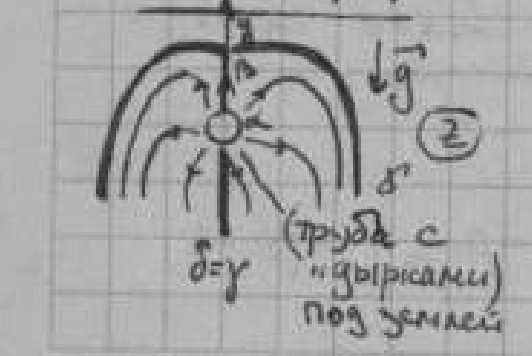
\includegraphics[width=.38\linewidth]{figures/notes-physical-domain.png}
\hspace{.04\linewidth}
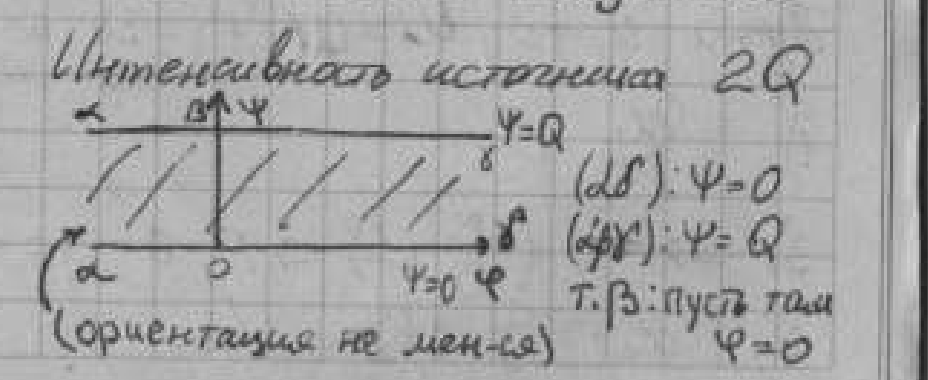
\includegraphics[width=.54\linewidth]{figures/notes-potential-domain.png}
\end{center}
Труба с «дырками» под землей.

\[
(\alpha\delta):\ \psi=0,\qquad(\beta\gamma):\ \psi=Q.
\]
Т. $\beta$: пусть там $\varphi=0$.

(ориентация не мен-ся)

% Источник: porous-lecture-notes.pdf; печатная страница: неизвестна; страница файла: 15; видимый рукописный номер разворота: 15
\begin{center}
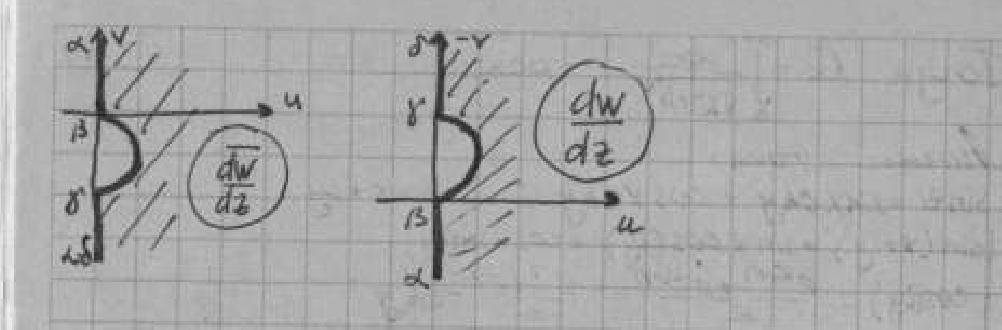
\includegraphics[width=.85\linewidth]{figures/notes-hodographs.png}
\end{center}
% На странице файла 15 включены только два рисунка-образа области течения, продолжающие постановку задачи на странице 14. Далее начинается «Гидравлическая теория ф-ции», не входящая в выбранный фрагмент.

\par\nobreak\smallskip{\small Рукописный конспект лекций, \texttt{porous-lecture-notes.pdf}, страницы файла 14--15, видимые рукописные номера разворотов 14 и 15. Автор, год, глава и параграф не указаны. Печатная нумерация не установлена.}
\end{textquote}
\end{document}
